\documentclass{beamer}

% Paquetes
\usepackage[spanish]{babel}
\usepackage[utf8]{inputenc}
\usepackage{subfig}
\usepackage{pifont}
\usepackage{amsmath}
\usepackage{bm}
\usepackage{commath}
\usepackage[backend=biber,style=numeric-comp,sorting=none]{biblatex}
% \usepackage{biblatex}
\addbibresource{xampl.bib}

% Tema de la presentación
\usetheme{Darmstadt}

% Configuraciones generales
\title{Bayesian Deep Learning}
\author{Jou-Hui Ho, Francisco Muñoz y José Villagrán}
\institute{
Facultad de Ciencias Físicas y Matemáticas\\
Universidad de Chile
}
\date{16 de diciembre de 2020}
% \logo{
\includegraphics[height=1.7cm]{presentaciones/img/logo solo ingenieria.jpg}}

%%%%%%% MACROS
% Letras en negrita
\newcommand{\bX}{{\bm{X}}}
\newcommand{\bY}{{\bm{Y}}}
\newcommand{\bW}{{\bm{W}}}
\newcommand{\bx}{{\bm{x}}}
\newcommand{\by}{{\bm{y}}}
\newcommand{\bb}{{\bm{b}}}
\newcommand{\bomega}{{\bm{\omega}}}
\newcommand{\fb}{{\bm{f}}}

% Letras rectas
\DeclareMathOperator{\ELBO}{ELBO}
\DeclareMathOperator{\KL}{KL}
\DeclareMathOperator{\VI}{VI}
\DeclareMathOperator*{\argmin}{arg\,min}

% Letras curvas
\let \oldL=\L
\renewcommand{\L}{\mathcal{L}}
\newcommand{\N}{\mathcal{N}}

% Letras bacanes
\newcommand{\esp}{\mathbb{E}}

\bibliography{../xampl}
% Inicio del documento
\begin{document}
% Portada
\frame{\titlepage}

% Tabla de contenidos
\AtBeginSection[]
{
\begin{frame}
    \nocite{*}
    \frametitle{Tabla de Contenidos}
    \tableofcontents[currentsection]
\end{frame}
}
% Resto de las diapos
\section{Motivación}
\begin{frame}{Motivación}
   \begin{itemize}[<+->]
       \item Los modelos de Deep Learning (DL) son \textbf{determinísticos}: estimaciones puntuales de parámetros y predicciones.
       \item Los modelos actuales de DL tienden a estar \textbf{sobreparametrizados}. Ej: GPT3 ($\sim$175 bill.) Y distintos parámetros pueden ajustarse bien en entrenamiento, pero arrojan resultados distintos en prueba. 
       \item No es posible saber si el modelo está prediciendo con certeza o solo adivinando.
       \item Relevante en áreas como medicina y vehículos autónomos.
       
       
   \end{itemize}
\end{frame}

\begin{frame}{Motivación}

    \uncover<1->{
        Ejemplo: softmax.
        \begin{center}
        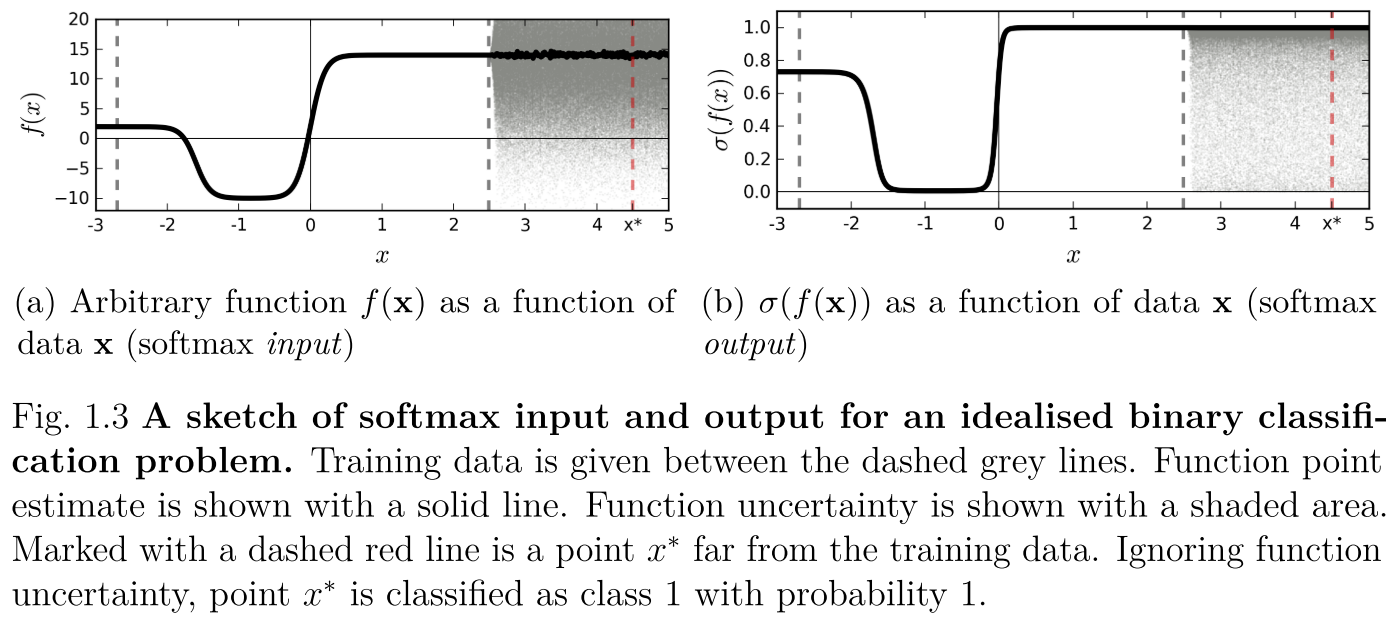
\includegraphics[height=4.5cm]{presentaciones/img/softmax.png}
        \end{center}
    } 

    \uncover<2->{
        \begin{alertblock}{Concepto erróneo}
            El output del modelo \textbf{no equivale} a la incerteza del modelo.
        \end{alertblock}
    } 

   
\end{frame}

\begin{frame}{Objetivo}
    Obtener la \textbf{incerteza} de una red neuronal, mediante un modelo que:
    \begin{itemize}
        \item sea escalable para datasets grandes,
        \item sea escalable para modelos complejos (CNN, RNN, etc.),
        \item use modelos ya existentes y
        \item sea fácil de entender y usar para personas no expertas.
    \end{itemize}
\end{frame}


%%%%%%%%%%%%%%%%%%%%%%%%%%%%%%%%%%%%%%%%%%%%%%%%%%%%%%%%%%%%%%%%%%%%%%
%%%%%%%%%%%%%%%%%%%%%%%%%%%%%%%%%%%%%%%%%%%%%%%%%%%%%%%%%%%%%%%%%%%%%%

\section{Modelamiento bayesiano}

\begin{frame}{Modelamiento bayesiano}
    Dadas las observaciones $X, Y$, tomar un \textbf{prior} sobre los parámetros $p(\omega)$ y encontrar los parámetros que \textbf{maximicen la posterior}:
    
    \begin{equation}
        p(\omega|X,Y) = \dfrac{p(Y|X,\omega)p(\omega)}{p(Y|X)},
    \end{equation}
    
    siendo $p(Y|X)$ la \textbf{evidencia}, dada por:
    
    \begin{equation}
        p(Y|X) = \int p(Y|X,\omega) p(\omega) d\omega.
    \end{equation}
    
    Sin embargo, en general esta integral no puede ser calculada analíticamente. Por lo tanto, se requiere una \textbf{aproximación}.
\end{frame}

\subsection{Inferencia variacional}

\begin{frame}{Inferencia variacional}


    \uncover<1->{
    Se define una \textbf{distribución variacional aproximada} $q_\theta(\omega)$ cuya estructura sea fácil de evaluar.
    
    \begin{equation}
        q^*_\theta(\omega) = \argmin_\theta \ KL\{q_\theta(\omega)||p(\omega|X,Y)\}
    \end{equation}
   } 

    \uncover<2->{
     Esto es equivalente a maximizar la \textbf{cota inferior de la evidencia (ELBO)}:
    \vspace{-5pt}
    \begin{equation}
        \text{ELBO}(q) = \mathbb{E}_{q_\theta(\omega)}\{\text{log} p(Y|X,\omega)\} - KL\{q_\theta(\omega)|| p(\omega)\} := \mathcal{L}_{VI}(\theta)
    \end{equation}
   } 
    
    \uncover<3->{
      \begin{exampleblock}{Ventajas}
        \begin{itemize}
            \item Balance: complejidad vs. ajuste de los datos.
            \item Captura la incerteza del modelo.
        \end{itemize}
    \end{exampleblock}
   } 
    
    
\end{frame}


%%%%%%%%%%%%%%%%%%%%%%%%%%%%%%%%%%%%%%%%%%%%%%%%%%%%%%%%%%%%%%%%%%%%%%
%%%%%%%%%%%%%%%%%%%%%%%%%%%%%%%%%%%%%%%%%%%%%%%%%%%%%%%%%%%%%%%%%%%%%%

\section{Bayesian Deep Learning}


\begin{frame}{Bayesian Neural Networks (BNN)}
    
    Se considera un prior sobre los pesos de la NN, induciendo una distribución sobre un conjunto paramétrico de funciones.
    
    
    \begin{align}
        \begin{split}
            \mathcal{L}_{VI}(\theta) &= \mathbb{E}_{q_\theta(\omega)}\{\text{log} p(Y|X,\omega)\} - KL\{q_\theta(\omega)|| p(\omega)\} \\
            &= \sum_{i=1}^N \mathbb{E}_{q_\theta(\omega)}\{\text{log} p(y_i|f^\omega(x_i))\} - KL\{q_\theta(\omega)|| p(\omega)\},
        \end{split}
    \end{align}

    siendo $f^\omega(x_i)$ el output del modelo para $x_i$.
    
    
    \begin{exampleblock}{Ventajas}
        \begin{itemize}
            \item Robustos a overfitting.
            \item Estimación de la incerteza.
            \item Puede aprender con datasets pequeños.
        \end{itemize}
    \end{exampleblock}
\end{frame}


\begin{frame}{Bayesian Neural Networks (BNN)}


    \uncover<1->{
        \color{red} \textbf{¡PERO!} \color{black} Esta expresión de $\mathcal{L}_{VI}(\theta)$:

        \begin{enumerate}
            \item requiere calcular sobre todo el dataset $\Rightarrow$ costoso, e
            \item intratable para modelos complejos (por ej. BNN con más de una capa).
        \end{enumerate}    
    } 
   
    \vspace{10pt}
    \uncover<2->{
        \color{green}
        \textbf{Solución:}
        \color{black}
        
        \begin{enumerate}[<+->]
            \item Usar minibatches.
            \begin{equation}
                \hat{\mathcal{L}}_{VI}(\theta) = \dfrac{N}{M}\sum_{i\in \mathcal{S}} \mathbb{E}_{q_\theta(\omega)}\{\text{log} p(y_i|f^\omega(x_i))\} - KL\{q_\theta(\omega)|| p(\omega)\}
            \end{equation}
            
            \item Usar estimadores Monte Carlo.
    \end{enumerate}    
    } 
   
\end{frame}


\subsection{Monte Carlo}

\begin{frame}{Monte Carlo}

    \uncover<1->{
    \textbf{Objetivo:}
    \begin{itemize}
        \item Estimar la esperanza de la log-likelihood.
        \item Estimar la derivada de la esperanza de la log-likelihood (c/r a $\theta$).
    \end{itemize}
   } 
    
    \vspace{10pt}
    \uncover<2->{
    Existen 3 estimadores:
    
    \begin{enumerate}
        \item Score function estimator
        \item Pathwise derivative estimator
        \item Characteristic function estimator
    \end{enumerate}
    }
    
    
\end{frame}

\subsection{Stochastic Regularization Techniques}

\begin{frame}{SRTs}
     \begin{block}{Interpretación}
        Optimizar \textbf{cualquier} NN con dropout es \textbf{equivalente} a una forma de inferencia aproximada: los pesos óptimos de un dropout NN son los mismos que los parámetros variacionales óptimos de una BNN con la misma estructura.
    \end{block}
\end{frame}


\subsection{Análisis}

\begin{frame}{Análisis}
    un analisis
\end{frame}



%%%%%%%%%%%%%%%%%%%%%%%%%%%%%%%%%%%%%%%%%%%%%%%%%%%%%%%%%%%%%%%%%%%%%%
%%%%%%%%%%%%%%%%%%%%%%%%%%%%%%%%%%%%%%%%%%%%%%%%%%%%%%%%%%%%%%%%%%%%%%

\section{Demo}

\begin{frame}{Demo}
    \begin{figure}[H]
        \centering
        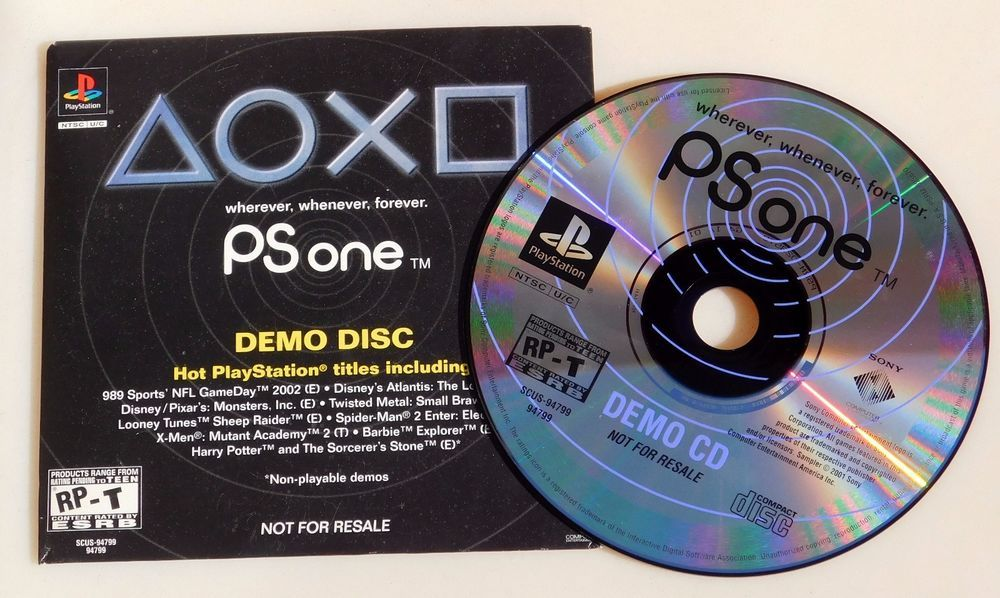
\includegraphics[scale=0.2]{presentaciones/img/demopsx.jpg}
        \caption{Psx Demo}
        \label{psx}
    \end{figure}
\end{frame}

\section{Conclusión}

\begin{frame}{Conclusión}
    conclusiones
\end{frame}


\begin{frame}{Conclusión}
    \centering
    \Huge ¡Gracias!
\end{frame}

\begin{frame}{Referencias}

\end{frame}

\begin{frame}{Tercera diapo}
    AQUÍ HAY MÁS INFO
     \begin{block}{Primer bloque}
        Aquí está el primer bloque
    \end{block}
    \begin{exampleblock}{Bloque de ejemplo}
        Aquí hay un bloque de ejemplo
    \end{exampleblock}
    \begin{alertblock}{Bloque de alerta}
        Aquí hay un bloque de alerta
    \end{alertblock}
\end{frame}


\begin{frame}[allowframebreaks]
    \frametitle{Referencias}
    \printbibliography
    % \bibliographystyle{amsalpha}
    % \bibliography{../xampl}
\end{frame}

\end{document}